\begin{figure*}
\centering
\setlength{\tabcolsep}{1pt}
{\small
\begin{tabular}{c c c c c c}
    \multicolumn{2}{c}{Objaverse original object} & \multicolumn{2}{c}{Shap-E} & \multicolumn{2}{c}{Sharp-It} \\
    %
    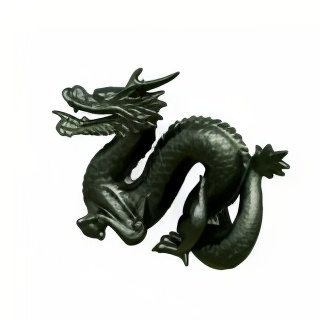
\includegraphics[width=0.15\linewidth, trim=50 0 50 0, clip]{images/supplementary/encode_decode/a_green_jade_objaverse/a_green_jade_objaverse_r1c1.jpg} &
    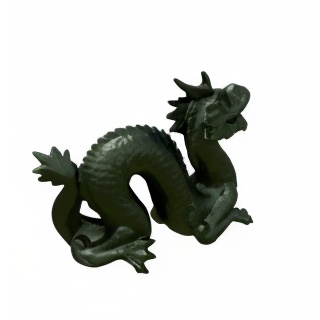
\includegraphics[width=0.15\linewidth, trim=50 0 50 0, clip]{images/supplementary/encode_decode/a_green_jade_objaverse/a_green_jade_objaverse_r2c1.jpg} &
    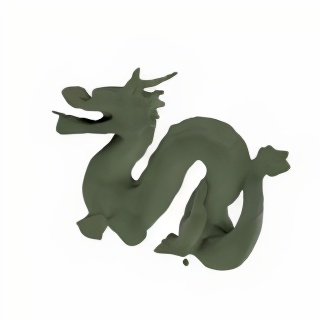
\includegraphics[width=0.15\linewidth, trim=50 0 50 0, clip]{images/supplementary/encode_decode/a_green_jade_dragon/a_green_jade_dragon_r1c1.jpg} &
    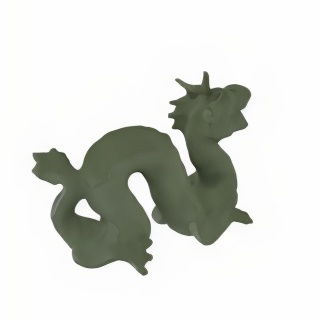
\includegraphics[width=0.15\linewidth, trim=50 0 50 0, clip]{images/supplementary/encode_decode/a_green_jade_dragon/a_green_jade_dragon_r2c1.jpg} &
    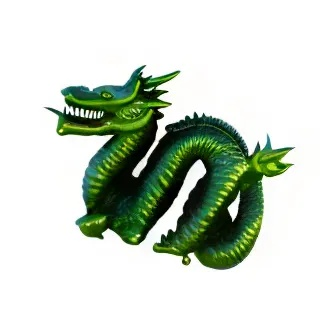
\includegraphics[width=0.15\linewidth, trim=50 0 50 0, clip]{images/supplementary/encode_decode/jade_dragon_sharp_it/jade_dragon_sharp_it_r1c1.jpg} &
    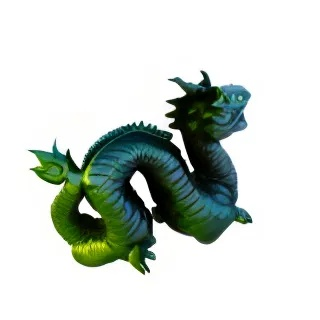
\includegraphics[width=0.15\linewidth, trim=50 0 50 0, clip]{images/supplementary/encode_decode/jade_dragon_sharp_it/jade_dragon_sharp_it_r2c1.jpg} \\
    \multicolumn{6}{c}{``A jade dragon statue''} \\
    %
    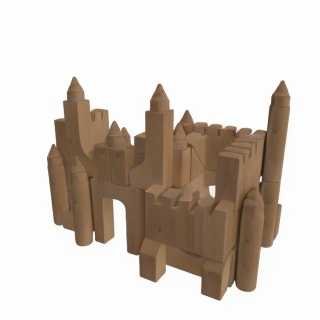
\includegraphics[width=0.15\linewidth, trim=50 0 50 0, clip]{images/supplementary/encode_decode/sand_castle_objaverse/sand_castle_objaverse_r1c1.jpg} &
    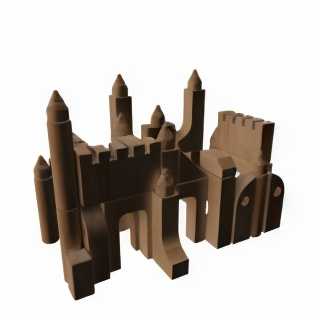
\includegraphics[width=0.15\linewidth, trim=50 0 50 0, clip]{images/supplementary/encode_decode/sand_castle_objaverse/sand_castle_objaverse_r2c1.jpg} &
    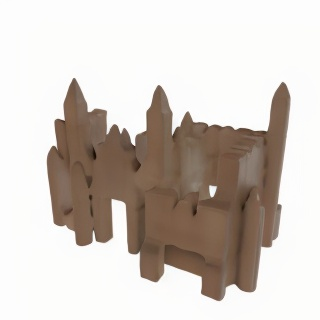
\includegraphics[width=0.15\linewidth, trim=50 0 50 0, clip]{images/supplementary/encode_decode/a_sand_castle/a_sand_castle_r1c1.jpg} &
    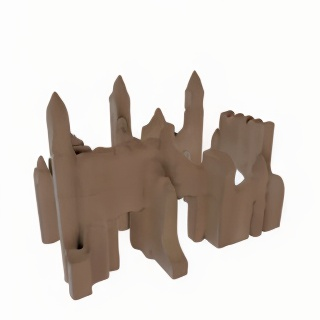
\includegraphics[width=0.15\linewidth, trim=50 0 50 0, clip]{images/supplementary/encode_decode/a_sand_castle/a_sand_castle_r2c1.jpg} & 
    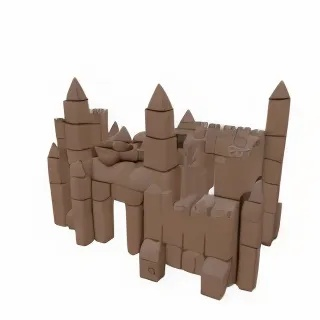
\includegraphics[width=0.15\linewidth, trim=50 0 50 0, clip]{images/supplementary/encode_decode/sand_castle_sharp_e/sand_castle_sharp_e_r1c1.jpg} &
    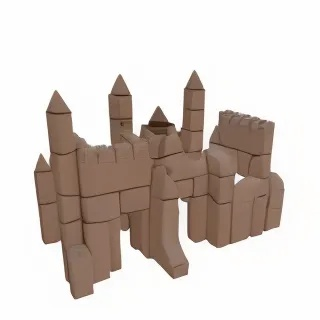
\includegraphics[width=0.15\linewidth, trim=50 0 50 0, clip]{images/supplementary/encode_decode/sand_castle_sharp_e/sand_castle_sharp_e_r2c1.jpg} \\
    \multicolumn{6}{c}{``A sand castle''} \\
    %
    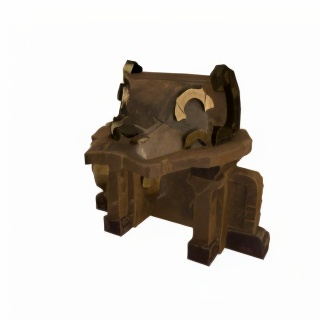
\includegraphics[width=0.15\linewidth, trim=50 0 50 0, clip]{images/supplementary/encode_decode/wooden_dog_original/wooden_dog_original_r1c1.jpg} &
    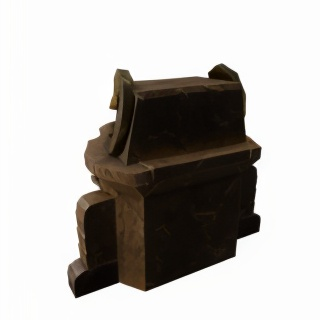
\includegraphics[width=0.15\linewidth, trim=50 0 50 0, clip]{images/supplementary/encode_decode/wooden_dog_original/wooden_dog_original_r2c1.jpg} &
    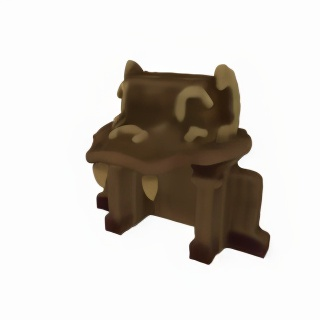
\includegraphics[width=0.15\linewidth, trim=50 0 50 0, clip]{images/supplementary/encode_decode/wooden_dog/wooden_dog_r1c1.jpg} &
    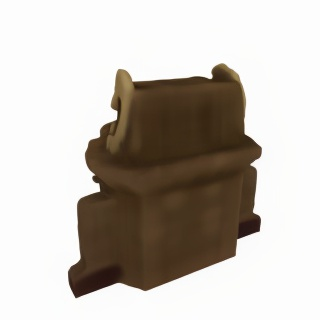
\includegraphics[width=0.15\linewidth, trim=50 0 50 0, clip]{images/supplementary/encode_decode/wooden_dog/wooden_dog_r2c1.jpg} &  
    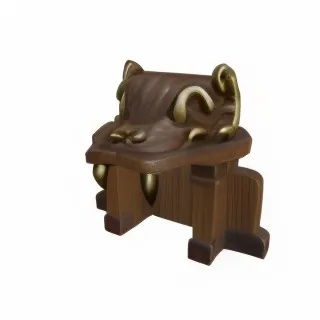
\includegraphics[width=0.15\linewidth, trim=50 0 50 0, clip]{images/supplementary/encode_decode/wooden_dog_sharp_it/wooden_dog_sharp_it_r1c1.jpg} &
    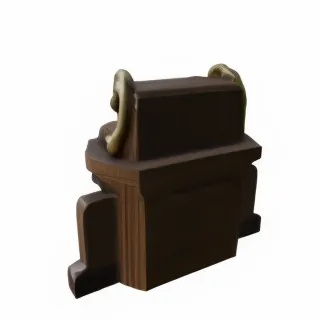
\includegraphics[width=0.15\linewidth, trim=50 0 50 0, clip]{images/supplementary/encode_decode/wooden_dog_sharp_it/wooden_dog_sharp_it_r2c1.jpg} \\
    \multicolumn{6}{c}{``A wooden dog statue''} \\
\end{tabular}
}
\vspace{-8pt}
\caption{
Example of high refinement quality of objects, from objaverse test set, where we encode the object into the Shap-E latent space, and refine it using Sharp-It}
\vspace{-12pt}
\label{fig:objaverse_encode}
\end{figure*}